%% SECTION HEADER /////////////////////////////////////////////////////////////////////////////////////
\section{Sample configuration}
\label{sec:sample}

%% SECTION CONTENT ////////////////////////////////////////////////////////////////////////////////////
The sample of interest was a \numproduct{500 x 500 x 1.5} \unit{\cubic\mm} unidirectional \ac{cfrp} plate with stack sequence \(\left[\ang{0},\,\ang{90}\right]_s\) bonded to an aluminium honeycomb core.
The volume fraction of fibres was assumed 47\%.
It was decided to use only one skin, as it is pictured in Fig.~\ref{fig:honeycomb}(b), with the intention of experimental validation and to be able to enlarge disbonds between the skin and the core located in the middle of the \ac{hsc} with a tool in a real sample. 
It was not decided to dedicate separate samples for each size of damage because too many factors would affect the signal value, including skin and sensors properties, the thickness of the adhesive layers, position of the core relative to the sensors, and distance between sensor.
Moreover, it renders closely the realistic scenario of monitoring the same structure.
\begin{figure}[H]
	\begin{center}
		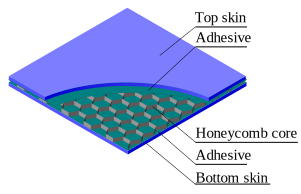
\includegraphics[width=0.95\textwidth]{Chapter_5/honeycomb}
	\end{center}
	\caption{Sample configuration: (\textbf{a}) top view of the sample, (\textbf{b}) \acf{hsc} and (\textbf{c}) details of the honeycomb cell.}
	\label{fig:honeycomb}
\end{figure}

The core geometry is accurately reproduced from the actual specimen, i.e., geometry of irregular hexagonal cells \(\left(\mathrm{h}_1 \ne \mathrm{l}_1\right)\) and double walls at the sheet joints, resulting from the core fabrication technology.
According to the drawing in Fig. \ref{fig:honeycomb}(\textbf{c}), the cell dimensions are \(\mathrm{w}_c\)=0.1 \unit{\mm}, h\(_1\)=11 \unit{\mm}, h\(_2\)=5 \unit{\mm}, l\(_1\)=10.4 \unit{\mm}, l\(_2\)=6 \unit{\mm} and the cell height g=14.5 \unit{\mm}.
The core was bonded to one \ac{cfrp} plate using the epoxy adhesive (Loctite EA3479B) with the thickness h\(_a\)=0.3 \unit{\mm}.
The adhesive layer covered the entire bottom surface of the skin.
\nomtypeR[w_core]{\(\mathrm{w}_c\)}{Core wall thickness}{}{\unit{\metre}}%
\nomtypeR[h_core]{h\(_1\), h\(_2\)}{Core cell length}{}{\unit{\metre}}%
\nomtypeR[l_core]{l\(_1\), l\(_2\)}{Core cell width}{}{\unit{\metre}}%
\nomtypeR[g_core]{g}{Cell height}{}{\unit{\metre}}%
\nomtypeR[h_adh]{h\(_a\)}{Adhesive layer thickness}{}{\unit{\metre}}%
\nomtypeR[h_pzt]{h\(_{PZT}\)}{Transducer thickness}{}{\unit{\metre}}%
\nomtypeG[phi_pzt]{\(\Phi_{PZT}\)}{Transducer diameter}{}{\unit{\metre}}%
\nomtypeR[h_glue]{h\(_g\)}{Cyanoacrylate glue thickness}{}{\unit{\metre}}%
Signal excitation and recording were accomplished with a pair of \acp{pzt}  (Noliac, NCE51) mounted to the top surface of the skin with cyanoacrylate glue.
The circular transducers of diameter \(\Phi_{PZT}\)=10 \unit{\mm} and thickness h\(_{PZT}\)=0.5 \unit{\mm} were attached 200 \unit{\mm} apart, as shown in Fig.~\ref{fig:honeycomb}(\textbf{a}).
The thickness of cyanoacrylate glue under \ac{pzt} was assumed to be h\(_g=50\) \unit{\micro\m}.

The material properties of the components assumed for the simulations are compiled in Tab.~\ref{tab:properties}.
The effective properties of the \ac{cfrp} skin were determined according to the rule of mixtures presented in the book by Vinson and Sierakowski \cite{vinson1993behavior}.
The authors provide a complete description of the homogenisation of composite properties.
Firstly, the stiffness matrix is determined for the single ply of the laminate along the fibre direction.
Then, the stiffness matrix is transformed for other orientations of the laminate plies by the transformation matrix composed of the direction cosines.
In the sample analysed, there are plies with an orientation of \ang{0} and \ang{90}.
Finally, all the plies in the laminate are homogenised through the thickness.
Explicit expressions of the stiffness components for the laminate modelled by solid elements are presented by Sun and Li in \cite{sun1988three}.
The comprehensive equations to derive the effective stiffness matrix are given in App.~\ref{app:eff_properties} and the resulting \ac{cfrp} properties are shown in Tab.~\ref{tab:properties_eff}.
\begin{table}[H]
	\centering
	\small
	\tabcolsep=0.25cm
	\caption{\label{tab:properties_eff} The homogenised mechanical properties of the \ac{cfrp} plate and the honeycomb core for +20\unit{\degreeCelsius}.}
	\begin{tabular}{ccccccccc}
		\toprule
		\multirow{2}{*}{\textbf{Material}} & \(\boldsymbol{E_{11}}\) & \(\boldsymbol{E_{22}}\) & \(\boldsymbol{E_{33}}\) & \(\boldsymbol{G_{12}}\) & \(\boldsymbol{G_{23}}\) & \(\boldsymbol{\nu_{12}}\)	& \(\boldsymbol{\nu_{23}}\) & \(\boldsymbol{\rho}\) \\
		& \unit{\giga\pascal} & \unit{\giga\pascal} & \unit{\giga\pascal} & \unit{\giga\pascal} & \unit{\giga\pascal} & -- & -- & \unit[per-mode = symbol]
		{\kilogram\per\cubic\metre}\\
		\midrule
		\ac{cfrp} & 69.5 & 69.5 & 8.16 & 3.43 & 2.96 & 0.03 & 0.37 & 1555\\
		laminate & & & & & & & &\\
		\midrule
		honeycomb & 0.007 & 0.005 & 2.76 & 0.002 & 0.86 & 0.999 & \(\approx0\) & 112\\
		core & & & & & & & &\\
		\bottomrule
	\end{tabular}
\end{table}
\nomtypeR[G]{\(G\)}{Shear modulus}{}{\unit{\giga\pascal}}%